%
% Metric Runtimes
%
\section{Metric Runtimes}

\subsection{UnweightedAllPairsShortestPathsR}
UnweightedAllPairsShortestPathsR is a metric runtime.

See plot: \ref{plot:RANDOM_100_500 - BARABASI_ALBERT_GROWTH_10_2.z.runtimes.2.metrics}, \ref{plot:RANDOM_100_500 - BARABASI_ALBERT_GROWTH_10_2.z.runtimes.2.metrics.CDF}.

%
% value table of UnweightedAllPairsShortestPathsR
%
\begin{tabular}{|l||l|}
\hline
	\textbf{Timestamp} & \textbf{Average} \\ \hline
	0 & 0.03453 \\ \hline
	1 & 0.00493 \\ \hline
	2 & 0.00548 \\ \hline
	3 & 0.00468 \\ \hline
	4 & 0.00511 \\ \hline
	5 & 0.00569 \\ \hline
	6 & 0.00876 \\ \hline
	7 & 0.01041 \\ \hline
	8 & 0.01123 \\ \hline
	9 & 0.01291 \\ \hline
	10 & 0.01413 \\ \hline
	11 & 0.01455 \\ \hline
	12 & 0.01571 \\ \hline
	13 & 0.01569 \\ \hline
	14 & 0.0201 \\ \hline
	15 & 0.01573 \\ \hline
	16 & 0.0172 \\ \hline
	17 & 0.0171 \\ \hline
	18 & 0.01899 \\ \hline
	19 & 0.02008 \\ \hline
	20 & 0.02381 \\ \hline
	21 & 0.02278 \\ \hline
	22 & 0.02351 \\ \hline
	23 & 0.02984 \\ \hline
	24 & 0.02829 \\ \hline
	25 & 0.02735 \\ \hline
	26 & 0.03388 \\ \hline
	27 & 0.03416 \\ \hline
	28 & 0.03968 \\ \hline
	29 & 0.04045 \\ \hline
	30 & 0.04222 \\ \hline
	31 & 0.05058 \\ \hline
	32 & 0.04639 \\ \hline
	33 & 0.04966 \\ \hline
	34 & 0.05202 \\ \hline
	35 & 0.05254 \\ \hline
	36 & 0.05371 \\ \hline
	37 & 0.06012 \\ \hline
	38 & 0.07029 \\ \hline
	39 & 0.06438 \\ \hline
	40 & 0.06862 \\ \hline
	41 & 0.07072 \\ \hline
	42 & 0.07137 \\ \hline
	43 & 0.07275 \\ \hline
	44 & 0.07371 \\ \hline
	45 & 0.07768 \\ \hline
\end{tabular}
\begin{tabular}{|l||l|}
\hline
	\textbf{Timestamp} & \textbf{Average} \\ \hline
	46 & 0.07947 \\ \hline
	47 & 0.08572 \\ \hline
	48 & 0.08776 \\ \hline
	49 & 0.0919 \\ \hline
	50 & 0.0921 \\ \hline
\end{tabular}

\subsection{DegreeDistributionR}
DegreeDistributionR is a metric runtime.

See plot: \ref{plot:RANDOM_100_500 - BARABASI_ALBERT_GROWTH_10_2.z.runtimes.2.metrics}, \ref{plot:RANDOM_100_500 - BARABASI_ALBERT_GROWTH_10_2.z.runtimes.2.metrics.CDF}.

%
% value table of DegreeDistributionR
%
\begin{tabular}{|l||l|}
\hline
	\textbf{Timestamp} & \textbf{Average} \\ \hline
	0 & 0.00163 \\ \hline
	1 & 7.3E-5 \\ \hline
	2 & 9.9E-5 \\ \hline
	3 & 1.15E-4 \\ \hline
	4 & 8E-5 \\ \hline
	5 & 1.21E-4 \\ \hline
	6 & 8.7E-5 \\ \hline
	7 & 1.38E-4 \\ \hline
	8 & 7.2E-5 \\ \hline
	9 & 7.3E-5 \\ \hline
	10 & 7E-5 \\ \hline
	11 & 9.6E-5 \\ \hline
	12 & 8.6E-5 \\ \hline
	13 & 9.2E-5 \\ \hline
	14 & 1.13E-4 \\ \hline
	15 & 9.1E-5 \\ \hline
	16 & 9.3E-5 \\ \hline
	17 & 7.8E-5 \\ \hline
	18 & 6.3E-5 \\ \hline
	19 & 1.07E-4 \\ \hline
	20 & 6.8E-5 \\ \hline
	21 & 7.1E-5 \\ \hline
	22 & 7.6E-5 \\ \hline
	23 & 7.5E-5 \\ \hline
	24 & 8.7E-5 \\ \hline
	25 & 7.5E-5 \\ \hline
	26 & 1.01E-4 \\ \hline
	27 & 6.2E-5 \\ \hline
	28 & 1.08E-4 \\ \hline
	29 & 6.7E-5 \\ \hline
	30 & 7.1E-5 \\ \hline
	31 & 1.17E-4 \\ \hline
	32 & 7.1E-5 \\ \hline
	33 & 8.7E-5 \\ \hline
	34 & 8.3E-5 \\ \hline
	35 & 8.2E-5 \\ \hline
	36 & 8.3E-5 \\ \hline
	37 & 1.49E-4 \\ \hline
	38 & 8.5E-5 \\ \hline
	39 & 1.8E-5 \\ \hline
	40 & 1.8E-5 \\ \hline
	41 & 2.1E-5 \\ \hline
	42 & 2.1E-5 \\ \hline
	43 & 2.2E-5 \\ \hline
	44 & 2.3E-5 \\ \hline
	45 & 2.1E-5 \\ \hline
\end{tabular}
\begin{tabular}{|l||l|}
\hline
	\textbf{Timestamp} & \textbf{Average} \\ \hline
	46 & 2.3E-5 \\ \hline
	47 & 2.1E-5 \\ \hline
	48 & 2.7E-5 \\ \hline
	49 & 2.6E-5 \\ \hline
	50 & 2.2E-5 \\ \hline
\end{tabular}

\subsection{UndirectedClusteringCoefficientR}
UndirectedClusteringCoefficientR is a metric runtime.

See plot: \ref{plot:RANDOM_100_500 - BARABASI_ALBERT_GROWTH_10_2.z.runtimes.2.metrics}, \ref{plot:RANDOM_100_500 - BARABASI_ALBERT_GROWTH_10_2.z.runtimes.2.metrics.CDF}.

%
% value table of UndirectedClusteringCoefficientR
%
\begin{tabular}{|l||l|}
\hline
	\textbf{Timestamp} & \textbf{Average} \\ \hline
	0 & 0.03503 \\ \hline
	1 & 0.0145 \\ \hline
	2 & 0.01062 \\ \hline
	3 & 0.00372 \\ \hline
	4 & 0.00319 \\ \hline
	5 & 0.00381 \\ \hline
	6 & 0.00417 \\ \hline
	7 & 0.00447 \\ \hline
	8 & 0.00455 \\ \hline
	9 & 0.00468 \\ \hline
	10 & 0.00483 \\ \hline
	11 & 0.00528 \\ \hline
	12 & 0.00543 \\ \hline
	13 & 0.00569 \\ \hline
	14 & 0.00649 \\ \hline
	15 & 0.00503 \\ \hline
	16 & 0.00592 \\ \hline
	17 & 0.00514 \\ \hline
	18 & 0.00522 \\ \hline
	19 & 0.00556 \\ \hline
	20 & 0.00541 \\ \hline
	21 & 0.00625 \\ \hline
	22 & 0.00594 \\ \hline
	23 & 0.00573 \\ \hline
	24 & 0.00661 \\ \hline
	25 & 0.00592 \\ \hline
	26 & 0.0071 \\ \hline
	27 & 0.00607 \\ \hline
	28 & 0.00759 \\ \hline
	29 & 0.00636 \\ \hline
	30 & 0.00679 \\ \hline
	31 & 0.0083 \\ \hline
	32 & 0.00671 \\ \hline
	33 & 0.00826 \\ \hline
	34 & 0.00797 \\ \hline
	35 & 0.00765 \\ \hline
	36 & 0.00786 \\ \hline
	37 & 0.00948 \\ \hline
	38 & 0.01117 \\ \hline
	39 & 0.00772 \\ \hline
	40 & 0.00765 \\ \hline
	41 & 0.0084 \\ \hline
	42 & 0.00814 \\ \hline
	43 & 0.00855 \\ \hline
	44 & 0.00888 \\ \hline
	45 & 0.00828 \\ \hline
\end{tabular}
\begin{tabular}{|l||l|}
\hline
	\textbf{Timestamp} & \textbf{Average} \\ \hline
	46 & 0.00832 \\ \hline
	47 & 0.00872 \\ \hline
	48 & 0.01059 \\ \hline
	49 & 0.0097 \\ \hline
	50 & 0.00903 \\ \hline
\end{tabular}

\subsection{Plots}

% plot z.runtimes.2.metrics
\begin{figure} [h]
	\centering
	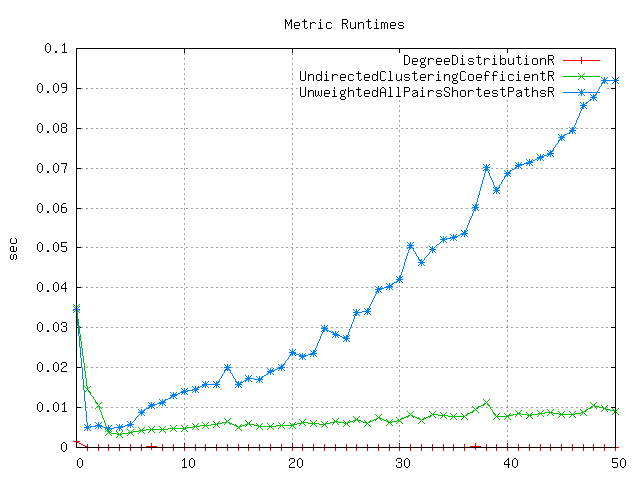
\includegraphics [scale=0.8] {plots/z.runtimes.2.metrics}
	\caption{z.runtimes.2.metrics}
	\label{plot:RANDOM_100_500 - BARABASI_ALBERT_GROWTH_10_2.z.runtimes.2.metrics}
\end{figure}

% plot z.runtimes.2.metrics.CDF
\begin{figure} [h]
	\centering
	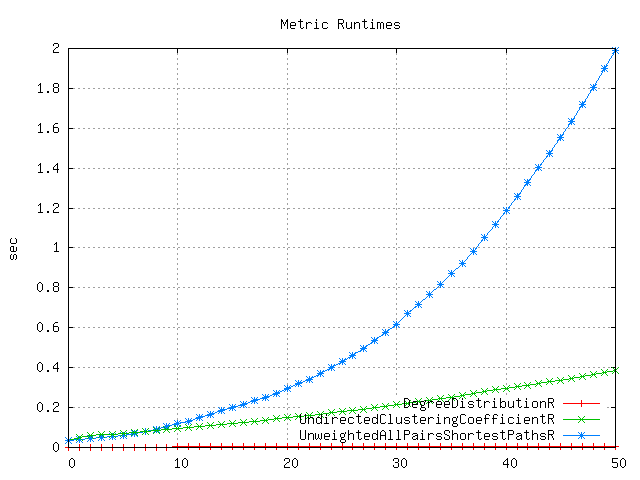
\includegraphics [scale=0.8] {plots/z.runtimes.2.metrics.CDF}
	\caption{z.runtimes.2.metrics.CDF}
	\label{plot:RANDOM_100_500 - BARABASI_ALBERT_GROWTH_10_2.z.runtimes.2.metrics.CDF}
\end{figure}


% end of document
